\documentclass[11pt]{article}

% arXiv cs.LG-compatible preamble: standard packages only, no exotic deps.
\usepackage[utf8]{inputenc}
\usepackage[T1]{fontenc}
\usepackage{amsmath,amssymb,amsthm}
\usepackage{graphicx}
\usepackage{booktabs}
\usepackage{tabularx}
\usepackage{seqsplit}
\usepackage{url}
\usepackage{hyperref}
\hypersetup{
  colorlinks=true,
  linkcolor=blue,
  citecolor=blue,
  urlcolor=blue,
  pdftitle={Grokking Modular Arithmetic under a Local, Backprop-Free Learning Rule: the Multiplicative-Character Basis as the Load-Bearing Ingredient},
  pdfauthor={Omar Bhular}
}
\usepackage[margin=1in]{geometry}

% Theorem environments
\newtheorem{theorem}{Theorem}
\newtheorem{proposition}[theorem]{Proposition}

\title{\textbf{Grokking Modular Arithmetic under a Local, Backprop-Free Learning Rule:\\ the Multiplicative-Character Basis as the Load-Bearing Ingredient}}
\author{Omar Bhular\\[2pt] {\small \texttt{omar@xmucane.com}}\\[2pt] {\small Independent}}
\date{August 10, 2026}

\begin{document}
\maketitle

\begin{abstract}
Backpropagation --- the algorithm behind modern deep learning --- is remarkably effective: it corrects a network's weights using a global error signal, once per pass, and it has powered the field's greatest successes. Local learning works differently: a synapse in the brain corrects itself using only what is around it --- no backpropagated derivative. We ask whether such a locally plastic, backprop-free rule can discover genuine mathematics, and we show that it can. A deep, sparsely-connected network, modeled on the cortex, is trained with a local rule called Equilibrium Propagation (EP). Training works in three steps: the network settles into its own natural pattern of activity, is gently nudged toward the correct answer, and learns from the difference between the two. The result is a striking learning curve: the network memorizes its training problems, then, suddenly, generalizes to problems it has never seen. Researchers call this phenomenon grokking. Our network groks modular arithmetic --- arithmetic on a clock face --- $7+6=13$ reads as 1 o'clock --- here with a 53-hour clock. It learns addition in eight of ten independent runs. Multiplication is the harder case, and the network learns it in all ten runs, reaching $\approx$99\% accuracy on never-seen problems. Why is multiplication harder? The network reads each number through a code --- and in our network that code is literally a set of wave patterns: every number is a chord, a set of tones. Addition's natural code is its harmonics (its Fourier basis) --- the same overtones that ring out on a plucked string. A single unit built from them cannot express multiplication: its best attempt fits the multiplication table with error 0.70, barely better than chance. A full layer has the aggregate capacity to fit the table, yet the local rule cannot discover that coordinated solution: it needs the right basis, not more capacity. Multiplication has its own alphabet of wave patterns --- the multiplicative characters --- waves stretched onto a logarithmic axis, on which multiplication reads as addition. Given that alphabet, the same local rule learns it. The rule is not magic: without a stabilization schedule, both operations grok-then-forget. To our knowledge, this is the first grokking of modular arithmetic under a locally plastic, backprop-free learning rule (search protocol in \S\ref{sec:related}).
\end{abstract}

\tableofcontents

\section{Introduction}\label{sec:intro}
The synapse's constraint --- learn only from what is around you --- rules out the algorithm behind modern deep learning. Backpropagation updates every weight using a global error signal computed by a backward pass through the network; a real neuron has no access to such a signal. This is the credit-assignment problem: attributing an error to the neurons that caused it. Can a network that learns only from local signals still discover genuine mathematics --- form the right internal structure, not just memorize data?

To test whether a learning rule forms correct internal structures rather than merely memorizing data, the standard probe is grokking \cite{power2022}: the sudden, late generalization to problems the network has never seen. Power et al.~\cite{power2022} showed that backprop-trained transformers grok modular arithmetic---including the modular product $x\cdot y \pmod{p}$---proving the probe is sharp enough to include a genuinely hard operation. What the network builds inside turns out to be a matter of representation. Nanda et al.~\cite{nanda2023} found that for addition the network represents numbers on a circle---a clock---and computes by rotating around it. Nguyen~\cite{nguyen2026} showed that for multiplication the load-bearing analysis basis is the discrete-log transform: the logarithmic axis on which multiplication reads as addition. The pattern across these results is that the code matters: a grokked network is one that found the right way to represent the operation. Throughout, ``code'', ``basis'', and ``alphabet of wave patterns'' name the same thing: the set of wave patterns through which the network reads its inputs. The additive Fourier basis---the harmonics that form addition's natural code---would seem the obvious representation for multiplication as well. It is not. As we prove in \S\ref{sec:theory}, the multiplication map needs the full rank-$(p+1)/2$ set of separable terms: a single unit's best attempt fails (error 0.70), and while a full layer has the aggregate capacity, the local rule cannot discover the coordinated solution. Multiplication needs its own alphabet of wave patterns on the logarithmic axis.

Yet for local, backprop-free rules---where each neuron updates only from the signals immediately around it---the analogous question has never been asked. To our knowledge, this gap has never been filled: no published work groks modular arithmetic under a locally plastic, backprop-free rule (search protocol in \S\ref{sec:protocol}). By ``locally plastic we mean that synaptic weight updates use only locally available activity and a teaching/error variable supplied through fixed random projections, not a backpropagated derivative. The major local rules have been tested almost entirely on vision benchmarks: equilibrium propagation \cite{scellier2017}, which learns by nudging a settled network toward the answer and comparing the two states; contrastive Hebbian learning \cite{hoier2023,hoier2024}, an earlier rule that also compares a free and a nudged phase, rooted in Hebb's ``neurons that fire together wire together''; and predictive coding \cite{sacramento2018}, in which each area predicts its input and learns from the mismatch. None of them asks whether a locally-learning network can find the right representation of an algorithmic operation---whether it can grok.

We built a deep predictive-coding network---several layers, each predicting the activity of the next---and trained it with equilibrium propagation. In this nudge-and-compare rule, the feedback connections are learned locally rather than copied from the forward weights (\S\ref{sec:background}). The network groks modular multiplication consistently across independent runs. The load-bearing ingredient is the alphabet of wave patterns on the logarithmic axis: when forced to use the harmonics of addition instead, the exact same network and rule fail. We prove the single-unit rank gap (\S\ref{sec:theory}) and report that the local rule does not discover the layer's coordinated solution (0/10; \S\ref{sec:falsified}).

\section{Background}\label{sec:background}
\paragraph{Why local rules matter.}
Local rules are compatible with energy-efficient compute-in-memory substrates (chips that compute inside the memory array itself), they bypass the symmetric-feedback bottleneck---backprop's backward pass needs the transpose of the forward weights, which local circuits cannot know---and the cortex demonstrably learns this way \cite{urbanczik2014,guerguiev2017,sacramento2018}. This compatibility comes at a real cost: equilibrium propagation settles for $T$ steps per update, requiring more compute per update than a single backprop pass on conventional hardware. Our engine's energy lever is therefore sparsity: a hard gate holds firing at roughly 10\%, so every settling step operates on sparse activations and structurally-sparse weights (the feedforward matrices are $\approx$9\% dense). Removing this gate destroys learning (\S\ref{sec:falsified}).

\paragraph{Equilibrium propagation and contrastive Hebbian learning.}
Equilibrium propagation (EP) \cite{scellier2017} trains a network by letting it settle into its own natural pattern of activity, nudging it toward the answer, and updating each weight by the difference between the two states---a contrastive update. Contrastive Hebbian learning (CHL) is its direct ancestor; dual-propagation \cite{hoier2023} accelerates CHL with dyadic neurons. Both are local (each unit uses only local pre/post activity) and backprop-free. On vision benchmarks these rules match or approach backprop \cite{hoier2023,hoier2024}. We use EP as the contrastive engine.

\paragraph{Dendritic predictive coding.}
Predictive coding (PC) treats each cortical area as minimizing a local prediction error \cite{raoballard1999}. Sacramento et al.~\cite{sacramento2018} showed that a PC network with apical/basal dendrites (the two input branches of a cortical neuron) implements an approximate backprop-like credit assignment using only local signals. Our engine's layer-0 dendritic products implement the addition theorem (see \S\ref{sec:theory}); the network is a sparse predictive-coding cortex in the PC family.

\paragraph{Oja weight mirroring (no weight transport).}
The symmetric-feedback (weight-transport) problem --- backprop's backward weights are the transpose of the forward weights, which local circuits cannot know --- is addressed by learning the feedback connection locally via Oja's rule \cite{oja1982}: a Hebbian-style update that aligns the feedback weights with the forward weights while keeping them normalized. Sacramento et al.~\cite{sacramento2018} established that the PC feedback converges to the transpose of the feedforward weights. In our engine, the C2 feedback connections $B_{\mathrm{fb}}$ are learned via a contrastive update, while a separate Oja-rule experiment (C11; see \S\ref{sec:nowt}) tests locally learned alignment, with partial, regime-dependent results.

\paragraph{Grokking and mechanistic interpretability.}
Grokking was identified by Power et al.~\cite{power2022}. Nanda et al.~\cite{nanda2023} reverse-engineered the addition circuit (the ``clock''); Nguyen~\cite{nguyen2026} showed that a transformer groks multiplication via a discrete-log clock and that the correct analysis basis is the multiplicative-character transform. The recent scaling analyses of deep predictive coding (Depth-$\mu$P \cite{innocenti2025}; PC-ALM \cite{seely2026}) establish that deep local PC can be made to train stably when correctly parameterized; they do not study arithmetic grokking.

\paragraph{Our engine's parameterization paradigm.}
Our $L=6$ engine follows the deep-PC parameterization lessons of Depth-$\mu$P \cite{innocenti2025} and PC-ALM \cite{seely2026}: our original $L=4$ configuration suffered what PC-ALM terms ``diffusive credit propagation'' (concentration of the error signal near the output), the failure mode it diagnoses at depth \cite{seely2026}. The $L=6$ engine adds the local three-factor/error architecture (each neuron's update combines pre-synaptic activity, post-synaptic activity, and a per-area error signal) and hard-gate sparsity that make depth work.

\paragraph{Scope of the novelty claim.}
Throughout, ``to our knowledge'' is bounded by the dated, reproducible search protocol in \S\ref{sec:related} (cutoff 2026-08-10, re-run before submission). The claim is negative-in-the-record, not impossible-in-principle: no published local-rule grokking of any modular-arithmetic task, addition or multiplication, was found.

\section{Methods}\label{sec:methods}
\subsection{Engine}\label{sec:engine}
The model is a deep ($L=6$) sparse predictive-coding cortex with a hard firing gate at 10\% (the fraction of active units after k-winners-take-all) and a per-area error architecture. Inputs are the $2d = 104$ features for $d = 52$: the cosine and sine of the character phases $\omega_k(a) = 2\pi k \log_g(a)/(p-1)$ and $\omega_k(b)$ for $k = 1, \dots, 26$; the bilinear products of these features are formed inside layer-0 by the dendritic circuit (\S\ref{sec:addition-theorem}). Learning uses a local three-factor contrastive update: each synapse combines pre-synaptic activity, a local apical error signal, and the contrastive (nudged minus free) difference,
\begin{equation}\label{eq:ep}
\Delta W_l = \frac{\eta_l}{\beta B}\left[X_l^{+\top}\epsilon_{l+1}^{+} - X_l^{-\top}\epsilon_{l+1}^{-}\right] - \lambda_W W_l,
\end{equation}
where $X_l^{\pm}$ is the pre-synaptic activity at layer $l$ in the nudged ($+$) and free ($-$) phases, $\epsilon_{l+1}^{\pm}$ is the post-synaptic apical error (see below), $B$ is the batch size, and $\beta$ is the EP contrast parameter. The apical error at each layer combines local feedback, a broadcast teaching signal, and a local prediction:
\[
\epsilon_l = B_{\mathrm{fb}}^{(l)} a_{l+1} + B_{\mathrm{hc}}^{(l)} r_{\mathrm{HC}} - P^{(l)} a_l,
\]
where $P^{(l)}$ is the local prediction matrix, $r_{\mathrm{HC}}$ is the hippocampal teaching signal (zero in the free phase, the target $Y$ in the clamped phase), projected to each area through fixed random matrices $B_{\mathrm{hc}}^{(l)}$. There is no backpropagated derivative, no weight transport, and no \texttt{torch.optim} in the learning track. Feedback connections $B_{\mathrm{fb}}$ are learned locally via a contrastive update (not copied from forward weights); a separate Oja-rule experiment (C11, \S\ref{sec:nowt}) tests locally learned feedback alignment.

\paragraph{Locality of every update.} Table~\ref{tab:locality} lists, for every parameter class, the information its update uses. No update uses a backpropagated derivative; the global quantities are the phase schedule (free/clamped), the scalar learning rates, and the output target error $r_{\mathrm{HC}}$ broadcast through fixed random matrices (no weight transport, no chained gradient).
\begin{table}[ht]
\centering
\small
\begin{tabular}{ll}
\toprule
Parameter & Update inputs \\
\midrule
Forward weights $W$ & pre-synaptic activity, post-synaptic activity, per-area error (EP contrastive) \\
Feedback mirror $W_{\mathrm{fb}}$ & locally learned via contrastive update (not Oja in C2; Oja tested separately in C11) \\
Thresholds $\alpha$ & local activity, homeostatic rate \\
Readout $W_{\mathrm{out}}$ & local EP contrastive signal \\
Encoder & fixed (given, not learned) \\
Global quantities & phase schedule (free/clamped), scalar learning rates; output target error $r_{\mathrm{HC}}$ broadcast through fixed $B_{\mathrm{hc}}$ --- no backpropagated derivative, no weight transport \\
\bottomrule
\end{tabular}
\caption{Locality audit: the information available to each update.}
\label{tab:locality}
\end{table}
Here ``per-area error'' denotes the error variable locally available to neurons within that area; it is not a broadcast scalar loss or a backpropagated derivative from the output.

\paragraph{Stabilization schedule C+D.}
Persistent grokking requires a step-decayed weight gain $\gamma_W = 0.5$ and a decayed threshold-adaptation rate $\gamma_\alpha = 0.25$, with decay timescale $T_{\mathrm{decay}} = 1500$ steps (``C+D'' names the two decayed quantities: the weight gain C and the threshold-adaptation rate D). These constants encode the homeostatic timescale-separation principle (threshold adaptation slow relative to weight updates; see \S\ref{sec:discussion}). The same rule and schedule grok addition and multiplication.

\subsection{Encoders}\label{sec:encoders}
\begin{itemize}
\item \textbf{Additive Fourier encoder $E_{\mathrm{add}}$ (period $p$):} the standard additive Fourier basis used for addition.
\item \textbf{Multiplicative-character encoder $E_{\mathrm{mult}}$ (period $p-1$):} built from the fixed discrete-log table $x = \log_g(a)$ with $g$ a primitive root mod $p$ (a number whose powers generate all nonzero residues). For $p=53$, $g=2$ (order $52=p-1$, verified). The table is a fixed periphery transform in this paper (the alphabet is given, not acquired; see \S\ref{sec:limitations}); follow-up work demonstrates the same alphabet is \emph{learned} under local rules (streaming Oja EC self-organization, alignment 1.0000 batch / 0.972 streaming).
\end{itemize}

\subsection{Training budget}\label{sec:budget}
Training budgets are reported per experiment (see Appendix~\ref{app:claims} for the per-claim ledger detailing state steps and $n_{\mathrm{col}}$, the number of readout columns used). We allocate 2000 steps for claims C1 and C7 (single column, no voting), 3000 steps for C2--C4, and 6000 steps for C8 and C9. All headline claims run across 10 independent seeds using a strict 80/20 train/test split, ensuring the test and train sets are entirely disjoint ($\mathrm{test} \cap \mathrm{train} = \emptyset$). The split is a single fixed permutation (drawn with seed 42) of the 2704 pairs $(a,b) \in \{1,\dots,52\}^2$ (zero excluded), shared across all seeds and both arms, so every condition sees identical data. Unequal step counts are disclosed explicitly and are never compared cross-experiment without explicit notification. Budgets are reported in optimizer steps: an EP update costs $T$ settling steps (here $T{=}10$), so equal optimizer-step budgets are not equal forward-compute budgets; the backprop comparison (\S\ref{sec:limitations}) is optimizer-step-matched.

\section{Theory: why the basis is load-bearing}\label{sec:theory}
\subsection{The addition theorem is bilinear}\label{sec:addition-theorem}
The layer-0 dendritic products in our engine implement the addition theorem
\begin{equation}\label{eq:addthm}
\cos(ka)\,\cos(kb) = \tfrac{1}{2}\left[\,\cos(k(a+b)) + \cos(k(a-b))\,\right],
\end{equation}
so once the input carries a cosine (additive-Fourier) basis of period $p$, the tone for $a+b \bmod p$ is manufactured inside the network by bilinear products of separable input features. This is why a bilinear/PC network is the natural home for addition.

\subsection{The rank gap: a small additive-Fourier layer cannot express multiplication}\label{sec:rankgap}
We make this precise in three steps: (i) a single neuron provably cannot express the multiplication map --- a rank argument (Theorem~\ref{thm:rankgap}); (ii) a full layer has the aggregate capacity to represent it --- verified numerically; (iii) the local rule nonetheless fails to find that coordinated solution on the wrong basis --- empirical, reported in \S\ref{sec:falsified}.

The multiplication table, viewed as a matrix, cannot be assembled from fewer than 27 simple row-times-column pieces; a single neuron supplies one such piece, which is why its best fit is near chance. Formally: let the multiplication map be $m(a,b) = \cos(kab)$ over $\mathbb{F}_p$ (or the corresponding target tone). The kernel mixes every additive character (each of the $p$ wave patterns $e^{2\pi i k a/p}$) into the product, and the gap is a precise rank statement: a bilinear layer (one whose output is a sum of products of input features) whose output is a sum of $m$ products of separable features $u_i(a)v_i(b)$ expresses only kernels of rank at most $m$ (each product is a rank-one matrix), so the number of units is a hard expressivity bound. Here ``rank'' counts the number of independent row-times-column pieces a matrix needs; a matrix of rank $r$ is exactly a sum of $r$ such pieces.

\begin{theorem}[Rank gap]\label{thm:rankgap}
For an odd prime $p$ and fixed tone $k \in \{1, \dots, p-1\}$, the multiplication kernel $K(a,b) = \cos(2\pi k ab / p)$ has rank exactly $(p+1)/2$. Consequently, no bilinear network with fewer than $(p+1)/2$ units over separable features expresses the multiplication map: a single unit's best rank-one fit attains RMSE (root-mean-square error) $\approx 0.70$ ($R^2 \approx 0.04$).
\end{theorem}

\begin{proof}
Rows $a$ and $p-a$ of $K$ coincide because $\cos$ is even, so the rank is at most $(p+1)/2$: the distinct rows are those indexed by $a = 0, \dots, (p-1)/2$. Conversely, row $a$ is the cosine mode $\cos(2\pi f_a b / p)$ with folded frequency $f_a = \min(ka \bmod p,\, p - ka \bmod p)$. The map $a \mapsto ka \bmod p$ is a bijection of $\mathbb{Z}_p$, so the folded frequencies of the rows $a = 0, \dots, (p-1)/2$ are pairwise distinct; distinct cosine modes over $\mathbb{Z}_p$ are orthogonal, hence the $(p+1)/2$ distinct rows are linearly independent. The rank is exactly $(p+1)/2$. The single-unit bound follows because each separable product $u_i(a)v_i(b)$ is a rank-one matrix and the rank of a sum is at most the number of terms.
\end{proof}

The best rank-1 separable approximation of the multiplication kernel fits $\cos(kab)$ with RMSE $\approx 0.69$ ($R^2 < 0.05$) over the nonzero domain --- a numerical instantiation of the rank gap (claim C5, Part (i); our own computation gives RMSE $0.686$ over $\mathbb{F}_p^\times$, $R^2 = 0.036$). The bound of Theorem~\ref{thm:rankgap} is per neuron, not per layer: any matrix of rank $r$ is a sum of $r$ rank-one terms, and $K$ has rank $(p+1)/2 = 27$ over the full field $\mathbb{F}_p$. The experimental encoder operates on $\mathbb{F}_p^\times$ (zero excluded: the discrete log is undefined at zero), where the restricted kernel has rank $(p-1)/2 = 26$. Thus the experiment's 1536-unit layer is well above the exact rank requirement. A full layer-0 with a rich feature set fits the map to RMSE $\approx 0.019$ ($R^2 \approx 0.999$). The layer therefore has no expressivity gap; it has a learnability gap --- Part (iii) of the roadmap above.

This capacity is theoretical, not reachable by the local rule. Realizing the kernel requires many neurons to coordinate their individual contributions toward a single shared target --- a distributed, high-rank composition --- and under equilibrium propagation with locally learned feedback, every weight updates from local pre-synaptic activity and apical error signals. No local signal was found that assigns each neuron its share of the multiplication map, and the rule, as tested, does not coordinate the ensemble toward such a factorization; empirically the network fails to grok in this basis (0/10; \S\ref{sec:falsified}). The local rule therefore does not discover the brute-force distributed solution: for local learning, the correct basis was an empirical prerequisite among the representations and training routes tested here, not an optimization shortcut.

Part (iii) is a proposition, not a theorem. We do not claim to have proven that a learning wall must exist for every conceivable architecture. The expressivity rank gap (Part (i), Theorem~\ref{thm:rankgap}) is rigorous; the learning wall (that the wrong basis cannot be overcome by training the encoder) is stated as a proposition supported by our learned-encoder falsifier and bounded by the acquisition question (\S\ref{sec:limitations}). Its empirical content is precisely the capacity-versus-discoverability distinction above: the layer has the terms to fit the map, yet no local signal coordinates them, so the local rule requires a suitable basis to function reliably in the configurations tested here.

\subsection{The character basis dissolves the gap}\label{sec:character}
\begin{proposition}[Log-domain reduction]\label{prop:log}
For a primitive root $g \bmod p$, the map $a \mapsto \log_g(a)$ is a bijection $\mathbb{F}_p^\times \to \mathbb{Z}_{p-1}$, and
\begin{equation}\label{eq:logred}
a \cdot b \equiv g^{\log_g a + \log_g b \bmod (p-1)} \pmod{p}.
\end{equation}
Multiplication mod $p$ is therefore addition mod $p-1$ in the log coordinate system.
\end{proposition}

This is verified exactly: $g=2$ has order $52 = p-1 \bmod 53$; the exp map's discrete Fourier transform error is $1.4\times 10^{-14}$; there are $0/140{,}608$ homomorphism violations and $0/2704$ product mismatches (claim C6).

\section{Results}\label{sec:results}
We report both the best and final accuracy for every claim, with state steps and $n_{\mathrm{col}}$ explicitly disclosed (Appendix~\ref{app:claims}). Figures F1--F6 (Appendix~\ref{app:figures}) are generated from the exact artifact paths listed there.

\subsection{Grokking and grok-then-forget (C1--C4)}\label{sec:grok}
A deep PC cortex successfully groks addition modulo 53, and with the multiplicative-character basis $E_{\mathrm{mult}}$ alongside the C+D stabilization schedule, multiplication modulo 53 groks persistently (Table~\ref{tab:grok}; Figure F1, Appendix~\ref{app:figures}).

Without stabilization, the network exhibits a catastrophic grok-then-forget dynamic: multiplication groks before collapsing entirely, and addition suffers a similar collapse (Table~\ref{tab:grok}). This grok-then-forget collapse is not multiplication-specific: we observe it for both addition and multiplication under the unstabilized configuration. Both operations exhibit the same qualitative grok-then-forget failure mode and recover under C+D stabilization, which restores stable high accuracy in both.

\begin{table}[ht]
\centering
\caption{Grokking and grok-then-forget (C1--C4): best and final accuracy, with seeds $\geq 0.90$ and means. Sources: \texttt{outputs/l6eqcap\_T10\_10seeds.json} (5ea8114); \texttt{outputs/basis\_swap\_v13\_mult-stab\_frac80\_L6\_N1536\_T10.json} (87c7250); \texttt{outputs/basis\_swap\_v13\_mult-nostab\_frac80\_L6\_N1536\_T10.json} (38c6702); \texttt{outputs/basis\_swap\_v13\_add-sanity\_frac80\_L6\_N1536\_T10.json} (38c6702).}
\label{tab:grok}
\small
\begin{tabularx}{\textwidth}{@{}lXXX@{}}
\toprule
Arm & Best & Final & Steps \\
\midrule
Add mod 53 (C1) & 10/10 $\geq 0.90$, mean 0.946 & 8/10, mean 0.924 & 2000, 1 col \\
Mult + C+D (C2) & 10/10 $\geq$ 0.90, mean 0.9998 & 10/10 $\geq$ 0.90, mean 0.989 $\pm$ 0.026 (median 0.997, min 0.917, max 1.000) & 3000 \\
Mult, unstabilized (C3) & 10/10, mean 0.966 & 5/10, min 0.124 & 3000 \\
Add, unstabilized (C4) & 10/10, mean 0.971 & 4/10, min 0.109 & 3000 \\
\bottomrule
\end{tabularx}
\end{table}

\paragraph{Terminology.} We distinguish \emph{peak-grok} (best accuracy $\geq 0.90$ at any step; best accuracy is the maximum test accuracy over all evaluations) from \emph{persistent-grok} (final-window mean $\geq 0.90$; the final-window mean is the mean test accuracy over the last $W{=}5$ evaluations, taken every 100 steps, i.e., the final 500 steps); \emph{grok-then-forget} is peak-grok with final window $< 0.90$ and a pre-specified drop (best $-$ final $\geq 0.03$). The distinction is load-bearing: unstabilized runs peak-grok 10/10 but persist 4/10 by the window definition (5/10 by final accuracy) (C3), while stabilized runs persist 9/10 by the window definition (10/10 by final accuracy) (C2). The C2 result also reproduced on five held-out seeds $\{100,\dots,104\}$, disjoint from all prior seeds (5/5 final $\geq 0.90$, mean 0.998; \S\ref{app:claims}).

\subsection{T-sensitivity is an EP signature, not a backprop property (C7)}\label{sec:tcliff}
The settling-time parameter $T$ controls the quality of the EP contrastive gradient estimate, and the network's ability to grok is sharply $T$-sensitive. For addition (2000 steps, 10 seeds), final accuracy versus $T \in \{1, 5, 10\}$ is $0.125$ (0/10), $0.182$ (0/10), and $0.924$ (8/10), respectively (Figure F3, Appendix~\ref{app:figures}). For multiplication (3000 steps; $T{=}1,5$: 3 seeds; $T{=}10$: C2, 10 seeds), the cliff occurs at lower $T$ and is complete: $T{=}1$ fails to grok (0/3; window mean $0.273$, $\sim$14$\times$ chance), $T{=}5$ groks ($0.959$, 3/3), and $T{=}10$ groks (window mean $0.975$; final mean $0.989$, C2). At $T{=}1$ the contrastive signal does not reach the hidden layers: the per-layer error norm $\mathrm{d}h$ is nonzero only in the output layer (layer 5 of 6), so the network cannot form the credit path the rule needs. Backpropagation has no settling-time axis: a backprop reference arm run at $T \in \{1,5,10\}$ is exactly T-inert (window mean $0.300$ at all three, 3 seeds; $T$ is a no-op for the BP path, so the runs are identical; artifact \texttt{\path{outputs/bp\_control\_arm1\_mult\_tcliff\_L6\_N1536.json}}). The T-cliff is therefore a characteristic consequence of the EP settling procedure, absent from the BP reference because BP has no settling-time parameter. The backprop reference arm (\S\ref{sec:limitations}) shows that within the same 3000-optimizer-step budget, backprop has not begun to grok mult on this substrate, consistent with a rule-level effect; the substrate's contribution is not fully disentangled (a 10{,}000-step extension across ten seeds reaches window mean $0.763 \pm 0.089$, 0/10 grok; artifact \texttt{\path{outputs/bp\_control\_arm1\_mult\_main\_L6\_N1536\_T10\_S10000\_n10.json}}).

\subsection{Locally learned feedback (C11)}\label{sec:nowt}
The C2 engine learns its feedback connections $B_{\mathrm{fb}}$ via a local contrastive update (not Oja's rule), avoiding weight transport. A separate experiment (C11) tests whether an Oja-rule update \cite{oja1982} can align the feedback mirror $W_{\mathrm{fb}}$ with $W_{\mathrm{out}}^\top$ in an idealized warmup regime; this is mechanistically distinct from the C2 learning loop. Its alignment with $W_{\mathrm{out}}^{\top}$ is partial and regime-dependent (artifact \texttt{\path{outputs/c11\_oja\_run\_artifact.json}}): during Oja-only warmup with forward weights frozen, $\cos(W_{\mathrm{fb}}, W_{\mathrm{out}}^{\top}) \to 0.999$ at 500 steps; under joint EP training the forward weights move and the mirror chases a moving target, settling near $\cos \approx 0.75$--$0.80$ (relative error $\approx 0.6$--$0.7$) at 1000--1500 steps. The fixed-point identity $W_{\mathrm{fb}}\,\mathrm{Cov}(h, h) = \mathrm{Cov}(y, h)$ is the Oja/Sacramento theory. The idealized whitened-regime math-check (whitening = decorrelating the hidden activities so each has unit variance) reaches $\cos \to 0.999$ (20-seed sweep, \texttt{\path{scripts/math\_check\_oja\_t06df28d0.py}}). But the real non-whitened substrate (k-winners-take-all, k-WTA, 10\% firing) leaves $\cos$ stuck near $0.05$ --- the whitening gap is an open empirical question, not a verified convergence. We therefore report C11 as directional alignment during warmup, with exact mirror convergence under joint training open.

\subsection{Co-grokking and the readout (C8--C9)}\label{sec:cogrok}
Two distinct schemas (addition mod 53 and addition mod 59) successfully co-grok within a single cortex, achieving 10/10 accuracy for both (mean $0.999$ each; 6000 steps; Figure F5, Appendix~\ref{app:figures}). A shared-readout variant fails completely (0/10), localizing the representational separation pressure to the readout layer. Caveat: Claim C8 confirms accuracy co-grokking only; disjoint-unit coexistence was not confirmed (C-index $\approx 0$, a unit-overlap measure; lesion 0-drop, removing a unit leaves accuracy unchanged), per the experimental specification.

\subsection{Replay benefit (C10)}\label{sec:replay}
A hippocampal-replay analog (replaying stored training patterns during a sleep-like phase) applied during interleaved wake/replay training significantly improves multiplication acquisition under the local rule, at 1600 steps per arm across four wake/replay blocks (10 seeds) (Oja: $+0.454$, one-sided Wilcoxon $p = 0.002$; tied: $+0.333$, one-sided $p = 0.001$, where ``tied'' means the feedback mirror is tied to the forward weights rather than learned by Oja's rule; Figure F6, Appendix~\ref{app:figures}). These reflect the corrected statistical values detailed in Appendix~\ref{app:claims}; the Oja comparison uses $n{=}9$ (seed 1's wake arms absent from the source log).

\subsection{Expressivity (C5, F4)}\label{sec:expressivity}
Figure F4 (Appendix~\ref{app:figures}) demonstrates the rank gap: the best rank-1 separable approximation of the multiplication kernel achieves RMSE $\approx 0.69$ ($R^2 < 0.05$), whereas a full layer-0 achieves an RMSE of $0.019$ ($R^2 = 0.999$). Crucially, despite the full layer possessing the theoretical capacity to approximate the function, the local learning rule fails to discover this distributed solution: we report that the network does not bypass the rank-1 separable gap when operating on the incorrect basis (0/10; \S\ref{sec:falsified}).

\section{Discussion}\label{sec:discussion}
\subsection{The paradox resolved}\label{sec:paradox}
The scalable, additive-shaped local engine fails on multiplication in the additive basis --- not because the rule is weak, but because the target function needs the full rank-$(p+1)/2$ set of separable terms: while a layer with at least 27 units has the aggregate capacity to reach that rank, the local rule, as tested, does not coordinate 27 units onto a shared factorization (Theorem~\ref{thm:rankgap}). The multiplicative-character input dissolves this paradox by translating multiplication into addition within log-coordinates, an operation the local rule already natively groks. The load-bearing ingredient is the basis, corroborated from an independent direction by the transformer mechanism analysis of \cite{nguyen2026}.

We are careful to distinguish our claim (the input encoding basis under a local rule) from Nguyen's (the analysis basis of a backprop transformer): complementary, not identical.

\subsection{Brain analogy}\label{sec:brain}
The brain does not present the cortex with raw input; it hands it a tuned periphery. The retina log-compresses luminance (Weber--Fechner), and the cochlea performs a Fourier analysis. A multiplicative-character encoder is exactly this kind of periphery transform: it is the cortical input the task demands, not a task-engineering trick that the cortex is assumed to recover from unstructured spikes.

\subsection{Toward a general learner: acquire-then-freeze}\label{sec:generallearner}
The input basis here is a fixed periphery transform --- the same class as the accepted Fourier encoder for addition and, biologically, the retina's log-compression and the cochlea's Fourier analysis. Acquiring the alphabet from unstructured input under local rules is the explicit follow-up that turns this controlled first step into a general learner; it is the subject of companion work. Local predictive coding can bootstrap alphabets from structured input (Rao \& Ballard \cite{raoballard1999} learned Gabor receptive fields --- oriented edge detectors --- from natural images; sparse coding \cite{olshausen1996}, representing input as few active features, likewise), and our learned-encoder falsifier failed because one-hot input (a single active unit per number, carrying no structure) offers no structure to exploit --- not because local rules cannot learn bases. We do not claim the alphabet here is learned.

\paragraph{Relation to continual learning.}
The stabilization C+D (timescale-separated homeostatic thresholds) and the replay benefit are the local-rule ingredients of a continual-learning story; together they suppress the grok-then-forget collapse and improve acquisition. We report them as engine properties, not as a full continual-learning claim.

\section{Related work}\label{sec:related}
\subsection{Search protocol (dated, reproducible)}\label{sec:protocol}
We searched arXiv (first-party pages and API), Google Scholar, OpenReview, bioRxiv, and PMLR\slash ICML\slash ICLR\slash NeurIPS proceedings for local-rule $\times$ modular-arithmetic combinations (cutoff 2026-08-10; re-run before submission). Query families spanned equilibrium propagation, contrastive Hebbian learning, predictive coding, target propagation, forward-forward, Hebbian/STDP (spike-timing-dependent plasticity, the classic local rule), energy-based, and biologically-plausible learning, crossed with grokking, modular arithmetic, addition, and multiplication; plus mechanism negatives (``PC grokking addition'', ``EP grokking addition'') and task enumerators (``grokking modular polynomials'', ``discrete log clock modular multiplication'').

\subsection{Result of the negative search}\label{sec:negative}
Both ``equilibrium propagation'' grokking and ``contrastive Hebbian'' grokking returned empty result sets --- a genuine gap signal, not a query failure (adjacent conjunctions returned rich results). To our knowledge, no published work groks any modular-arithmetic task under a locally plastic, backprop-free rule. This is bounded by the protocol and dated.

\subsection{Grokking beyond transformers}\label{sec:grokking-beyond}
Grokking is not confined to transformers. Gromov~\cite{gromov2023} reproduced the phenomenon in a two-layer MLP on modular arithmetic, showing that delayed generalization is a property of the training dynamics, not of the attention architecture; Doshi et al.~\cite{doshi2024} extended this to modular polynomials and gave an analytical account of the grokking transition. Both are backprop-trained; we include them because they establish that the phenomenon we probe is not architecture-specific, and that the modular-arithmetic setting transfers across model classes --- while leaving the local-rule cell empty.

\subsection{The field table}\label{sec:fieldtable}
\begin{table}[ht]
\centering
\caption{Verified field table. The gap cell --- modular arithmetic $\times$ local (EP/CHL/PC) rule --- is empty in the published record. ``Local rules with gradient descent'' in some rule-learning literature \cite{zunkovic2024} uses ``local'' to mean data-local teacher-model learning (statistical-mechanics theory), not biologically-plausible local learning; we do not cite it as a local-learning prior.}
\label{tab:field}
\small
\begin{tabularx}{\textwidth}{@{}XXp{3.6cm}XX@{}}% artifact column fixed-width so \seqsplit wraps cleanly
\toprule
Work & Method & Task & Groks mult? & Local rule? \\
\midrule
Power et al. 2022 \cite{power2022} & Transformer+wd, mod $p$ incl. $x\cdot y$ & modular arithmetic & Yes (mult within) & No (BP) \\
Gromov 2023 \cite{gromov2023} & 2-layer MLP & modular arithmetic & Yes & No (BP) \\
Doshi et al. 2024 \cite{doshi2024} & MLP (analytical+BP) & modular multiplication & Yes & No (BP) \\
Nguyen 2026 \cite{nguyen2026} & Transformer, $a\cdot b \bmod 113$ & modular multiplication & Yes & No (BP) \\
H\o{}ier et al. 2023 \cite{hoier2023} & Dual Prop.\ (CHL/EP) & \seqsplit{MNIST/CIFAR100/ImgNet32} & n/a (vision) & Yes (CHL) \\
H\o{}ier \& Zach 2024 \cite{hoier2024} & Single-phase CHL & vision benchmarks & n/a (vision) & Yes (CHL) \\
Lv et al. 2025 \cite{lv2025} & Dendritic local learning & image benchmarks & n/a & Yes (local) \\
\midrule
\textbf{This work} & EP, sparse PC (locally learned feedback) & mult mod 53 & Yes (10/10) & Yes \\
\bottomrule
\end{tabularx}
\end{table}

\section{Conclusion}\label{sec:conclusion}
To our knowledge, we report the first grokking of modular arithmetic under a locally plastic, backprop-free learning rule. A deep sparse predictive-coding cortex trained with EP local updates groks modular multiplication persistently (10/10, mean 0.989) given a multiplicative-character input basis; it does not with the additive-Fourier basis, and we prove why (a rigorous rank gap). The discrete-log relabeling is the load-bearing ingredient, and the stabilization schedule that makes grokking persistent is a general engine property. We report honestly: in this paper the alphabet is given, not acquired (follow-up work demonstrates local-rule acquisition; see \S\ref{sec:limitations}); co-grokking is accuracy-only; the replay result is a single configuration; and EP's $T$-sensitivity is an EP-specific signature.

\section{Falsified alternatives}\label{sec:falsified}
We systematically falsified the alternative explanations for multiplication's failure --- partial-view routing (feeding each readout only part of the input), encoder learning, capacity, local structure, temporal credit (eligibility traces), and the additive-Fourier basis --- isolating the multiplicative-character basis plus stabilization as sufficient, and necessary among the tested alternatives. Among the representations tested, the multiplicative-character basis was necessary for reliable multiplication grokking under the tested local learning dynamics (the additive-Fourier basis cannot); stabilization C+D is necessary for persistent grokking (it prevents grok-then-forget, a general engine property affecting addition equally). The two are necessary for different properties; neither alone suffices for the full result.

\begin{table}[ht]
\centering
\caption{Falsified-alternatives table. Each row is an alternative explanation for multiplication's failure that we tested and ruled out; ``FALSIFIED'' means the route does not grok, ``BANKED NEGATIVE'' means it groks only transiently, and the control rows show what a working route looks like. The PC-vs-BP row is a killed comparison branch (pre-registered exit), not a falsified route. Two rows are flagged for the reader: the two-scale row is ``construction-broken'' (its add-sanity control failed), and the ``additive-Fourier + stabilization'' row is closed: the additive-Fourier basis on multiplication is falsified by the matched arm (\texttt{outputs/matched\_mult\_L6\_N1536\_T10.json}, 0/10, finals 0.07--0.09); the C+D schedule prevents post-grok collapse, not non-grok, so the stabilized variant was not separately run (disclosed in the row).}
\label{tab:falsified}
\small
\begin{tabularx}{\textwidth}{@{}XXp{3.8cm}X@{}}% artifact column fixed-width so \seqsplit wraps cleanly
\toprule
Route & Artifact (commit) & Result & Status \\
\midrule
HS hard-split partial-view voting & \texttt{\path{tbt\_laminar\_L6\_N512\_opt\_hsfvss.json}} cond=HS (103ce2e) & 0/10 (final mean 0.284, chance 0.019) & FALSIFIED \\
SS soft-split partial-view voting & same file cond=SS (103ce2e) & 0/6 (final mean 0.377) & FALSIFIED \\
FV full-view voting & same file cond=FV (103ce2e) & 10/10 GROK (final med 0.938) & POSITIVE control, not a negative \\
CC3 full-view no-voting (control) & \texttt{\path{tbt\_laminar\_L6\_N512\_opt.json}} + \texttt{\path{TBT\_LAMINAR\_FINAL\_LEDGER\_t\_5bfe1989.json}} & 9/10 final mean 0.939 & Positive control \\
Linear encoder from one-hot input & \texttt{\path{learned\_enc\_L6\_1\_s0-1-2.json}} (2df27ca) & 0/3, final mean 0.011 (chance 0.019) & Failed under tested configuration (one-hot carries no structure for a linear encoder to exploit) \\
Neighborhood size (10/20/35\% firing) & \texttt{\path{neighborhood\_sweep\_stage0.json}} (0899333) & flat 0.048 & FALSIFIED (capacity not the wall) \\
Two-scale local structure & \texttt{\path{two\_scale\_L6\_stage0.json}} (eedfc17) & 0.043 (C$\cdot$C floor 0.0427); add-sanity 0.004 & FALSIFIED (construction-broken) \\
Fourier basis on mult (2$\times$2 falsifier) & \texttt{\path{matched\_mult\_L6\_N1536\_T10\_alignment.json}} (c0ba6cd) & 0/10; align $<$ perm95 & FALSIFIED (representable, not locally learnable; alignment/permutation probe of the same run) \\
Additive Fourier on mult & \texttt{\path{outputs/matched\_mult\_L6\_N1536\_T10.json}} (c0ba6cd) & 0/10, finals 0.07--0.09 ($\approx$4$\times$ chance 0.019, far below the 0.90 grok threshold) & FALSIFIED (representable, not locally learnable; the C+D schedule prevents post-grok collapse, not non-grok, so the stabilized variant was not separately run) \\\\
Temporal eligibility-trace credit v14.4/14.5 & \texttt{\path{results\_v14\_temporal\_dendritic\_v3\_N4096\_L2.json}} (5c39677) & 0/10, Gate T2 $\approx 0$ & FALSIFIED (temporal credit dead route) \\
PC-vs-BP branch & \texttt{\path{docs/KILL\_CRITERION\_PC\_branch.md}} (8440d1d) & KILLED/CLOSED (pre-registered exit) & CLOSED (pre-registered exit; not a falsified route) \\
c3\_dynamic / AdamW-era engine & \texttt{\path{scripts/schema\_gate2.py}} (920a352/8fa1713) & REJECTED --- its mult-grok is AdamW (=BP), not the local EP rule & EXCLUDED (file exists at both cited commits; AdamW default verified in \texttt{\_optimizer}) \\\\
v13 line L=4 deep-freeze & \texttt{\path{v13\_14\_L4\_clamped\_seeds5-10.json}} (233f0a1) & 0/5 grok (deep-layer death) & FALSIFIED (L=4 wall) \\
Smoothgate Step 0 (no hard gate) & \texttt{\path{smoothgate\_step0\_L2.json}} (0ce2a25) & 0/10, final 0.043 & FALSIFIED (hard gate load-bearing) \\
Smoothgate re-verify ($\beta$=12 + hard gate) & \texttt{\path{smoothgate\_step0\_L2\_beta12.json}} (be37982) & 2/10 final but 10/10 peaked 0.97+ & BANKED NEGATIVE (grok-then-forget universal) \\
Character basis + stabilization \textit{(control --- not a falsified route)} & \texttt{\path{basis\_swap\_v13\_mult-stab\_frac80\_L6\_N1536\_T10.json}} (87c7250) & 10/10 final $\geq 0.90$ mean 0.989 & WORKS (control row, shown for contrast only) \\
\bottomrule
\end{tabularx}
\end{table}

\section{Limitations}\label{sec:limitations}
\begin{itemize}
\item \textbf{The alphabet is given, not acquired.} $E_{\mathrm{add}}$ and $E_{\mathrm{mult}}$ are hand-tuned fixed tables ($\varphi(a)=a$; $\varphi(a)=\log_2 a$). The network learned the operation, never the alphabet. This is task-specific engineering; acquisition under local rules from unstructured input was open at the time of this paper's experiments. \emph{Update (2026-08-13):} follow-up work demonstrates the alphabet \emph{is} acquired under local rules — a streaming Oja EC module self-organizes the same multiplicative-character basis (batch-limit alignment 1.0000, streaming 0.972) and tracks a rotating eigenspace (0.918 vs 0.327 frozen); a phi-matters control confirms the alphabet is load-bearing at depth (real 10/10 vs shuffled/random/one-hot 0/10). Acquisition from fully unstructured input (e.g. raw language) remains open (see \S\ref{sec:generallearner}).
\item ``To our knowledge'' is bounded by the dated search protocol (\S\ref{sec:related}); it is not ``no one can.''
\item C1 final 8/10, reported as-is. C8 is accuracy-only (disjoint-unit coexistence not confirmed). C10 uses corrected numbers ($+0.454$ Oja / $+0.333$ tied) with a documented data-quality caveat ($n=9$ for the Oja comparison).
\item The 80/20 pairwise split tests held-out input pairs, not held-out operands: the network sees many pairs involving each operand during training. Stronger compositional generalization (held-out operands) is left for future work.
\item Hard-gate sparsity (10\%) is load-bearing: the smooth-gate variant fails, and the 10\% hard gate is required.
\item Scale: $N=1536$, $L=6$ only; single prime $p=53$ for the headline result. The prime/size sweep (artifact \texttt{\path{outputs/prime\_sweep\_summary.json}}, 6196ed0) probes the boundary: $p{=}53$ at $N{=}1536$ groks (8/10 window, 10/10 best, mean window 0.948); crossing-point probes localize the wall: $p{=}29$ and $p{=}41$ both grok 10/10 at $N{=}1536$/3000 steps (window medians 0.991 and 0.994; artifacts \texttt{\path{outputs/p97wall\_I1\_p29\_N1536\_S3000.json}} and \texttt{\path{outputs/p97wall\_I2\_p41\_N1536\_S3000.json}}, f4a7791), so the boundary lies in $p \in (41, 97]$; $p{=}97$ at $N{=}1536$ does not grok within budget (0/10 window, 1/10 best, mean final 0.826). The failure appears primarily learnability-related, although a residual parameterization/capacity contribution cannot be completely excluded: by Theorem~\ref{thm:rankgap} the required rank is $(p{+}1)/2{=}49$, far below the layer's $N{=}1536$ units, so the layer has ample capacity to represent the table; the failure is the local rule's inability to coordinate the larger solution. A dedicated probe confirms this: even at 2.67$\times$ the budget (8000 steps, 10 seeds) the network does not grok (0/10, best 0.833; artifact \texttt{\path{outputs/p97wall\_D2\_p97\_N1536\_S8000.json}}, cb14e16), and the input-dimension accounting (in\_dim 192 for period 96) leaves layer-0 with 448$\times$ the required bilinear-product capacity (verdict \texttt{\path{docs/PROBE\_P97\_LEARNABILITY\_VS\_CAPACITY\_VERDICT.md}}, b200be2; a soft parameterization signal $R_{\mathrm{cap}} = N/((p{-}1)/2)^2 = 0.667$ (MARGINAL in the probe's three-zone model) leaves a minor capacity contribution not fully excluded). $p{=}97$ at $N{=}512$ is parameterization-limited: 0/10 grok, mean 0.283 --- 27$\times$ chance (chance $= 1/97 \approx 0.010$) but far below the 0.90 grok threshold. $R_{\mathrm{cap}}{=}0.222$ (HARD-FAIL) is a soft width heuristic, not the Theorem~\ref{thm:rankgap} rank bound (49 $\ll$ 512, so the layer is not rank-insufficient), and the test trajectory is still climbing at budget end --- the same learnability caveat as $N{=}1536$ applies. The sweep's $p{=}53$ final rate (9/10 $\geq 0.90$, mean 0.973) uses a different seed set than C2 (10/10); the sweep metric is the window average, stated explicitly to avoid an apparent inconsistency.
\item \textbf{Backprop control arm (substrate-scoped).} A backprop-trained equivalent (AdamW, cross-entropy, same L=6 architecture, same $E_{\mathrm{mult}}$ basis, same 3000-optimizer-step budget, 10 seeds) does not grok multiplication. The negative is budget-matched, not an impossibility claim, and it is specific to this substrate (the L=6 sparse cortex): backprop-trained transformers grok modular multiplication in the literature (Power et al.~\cite{power2022}; Nguyen~\cite{nguyen2026}).
\begin{itemize}
\item \emph{Budget-matched result:} 0/10 grok, mean final 0.347 (artifact \texttt{\path{outputs/bp\_control\_arm1\_mult\_main\_L6\_N1536\_T10.json}}, d9ff257). 3000 steps is far below the budgets at which backprop grokking of modular arithmetic is typically reported ($10^5$--$10^6$ optimization steps; Power et al.~\cite{power2022} report grokking at $10^5$ steps for the group product and $\approx 10^6$ for modular division).
\item \emph{Architecture confound:} a dense (gate-free) MLP control on the same data and basis does grok under backprop, at $\approx$3900 steps in a 20{,}000-step run (artifact \texttt{\path{outputs/rca\_e1\_dense\_mlp\_h512\_nh2\_relu\_wd1.0\_S20000.json}}, f6a750b; 3 seeds --- an existence proof, reported at lower confidence than the $n{=}10$ arms). The dense control varies both the learning rule and the architecture (dense MLP vs.\ sparse L=6 cortex) relative to the EP arm; the E2 extension (the extended-budget backprop run below) likewise varies architecture as well as sparsity, so the delay is attributed to the sparse L=6 substrate as a whole (isolating sparsity from architecture is open).
\item \emph{Extended budget:} a 10{,}000-step run on the actual sparse substrate (3.3$\times$ the budget, 10 seeds) reaches window mean $0.763 \pm 0.089$ (final mean $0.760 \pm 0.090$, best accuracies 0.63--0.94; 0/10 persistent grok at the 0.90 bar; artifact \texttt{\path{outputs/bp\_control\_arm1\_mult\_main\_L6\_N1536\_T10\_S10000\_n10.json}}, ddda769): backprop has not grokked by 10{,}000 steps on any of ten seeds. Three seeds peak-grokked transiently (0.922, 0.935, 0.933) --- grok-then-forget instances per \S\ref{sec:grok} --- before declining; one seed (0) plateaued near 0.60 (best 0.634 at step 6900, final 0.601), and the remaining six climbed to finals 0.69--0.84 --- consistent with a delay relative to the dense control ($\approx$3900 steps), magnitude not quantified, and eventual grokking at longer budgets remains open. The matched-architecture comparison (backprop on the sparse L=6 substrate at extended budget) is this E2 extension.
\item \emph{This isn't a handicap:} the straight-through estimator used here favors backprop (a standard trick that passes gradients through a non-differentiable gate as if it were the identity, giving backprop a full-rank gradient through the hard gate), so the comparison is tilted in backprop's favor; the local rule's win is not an artifact of a handicap. A memory-boundedness fix to the engine's alphabet-acquisition wrapper postdates the earliest BP runs; the BP control script is standalone and was not modified, so no number in this paper is affected by it.
\item \emph{Optimization regime:} the budget-matched backprop arm and the EP arm differ in batch protocol: backprop uses full-batch updates (all 2163 training pairs per step, AdamW with weight decay $\lambda{=}1.0$), while EP uses mini-batch updates (128 pairs per step). An exploratory sweep on the same sparse substrate at mini-batch 128 (1 seed, 3000 steps) grokked at $\lambda{=}1.0$ (window 0.952, grok step 1600) but not at $\lambda{=}0.1$ (window 0.850) --- consistent with the classic result of Power et al.~\cite{power2022} that weight decay enables grokking, and showing that under mini-batch with weight decay, backprop does grok on this substrate (artifact \texttt{\path{outputs/e4\_wd\_sweep\_bp\_arm.json}}, 0a1dc29; exploratory, not pre-registered).
\item \emph{The claim, precisely:} not ``local beats backprop''; on this substrate, with matched seeds and optimizer-step budget, the local rule groks where the full-batch backprop reference has not begun. EP groks mult in 3000 optimizer steps where full-batch BP on this substrate has not grokked within the same 3000-optimizer-step budget (the two arms differ in batch protocol --- full-batch 2163 for BP vs.\ mini-batch 128 for EP --- so the budgets are optimizer-step-matched, not forward-compute-matched; under mini-batch with weight decay, backprop also groks, see above).
\end{itemize}
\item \textbf{C11 is partial.} The Oja mirror aligns during warmup ($\cos \to 0.999$ at 500 steps) but exact convergence under joint training is not established on the real substrate (whitening gap; see \S\ref{sec:nowt}).
\item \textbf{C+D schedule grid.} The reported schedule ($\gamma_W=0.5$, $\gamma_\alpha=0.25$, $T_{\mathrm{decay}}=1500$) is one point of a boundary grid measured with 8 seeds per cell ($\gamma_W \in \{0.3,0.5,0.7\}$, $T_{\mathrm{decay}} \in \{750,1500,3000\}$): 5/9 cells sustain grokking; $T_{\mathrm{decay}}=3000$ collapses at all three $\gamma_W$, and $\gamma_W=0.7$ with $T_{\mathrm{decay}}=1500$ also forgets. The reported schedule ($\gamma_W=0.5$, $T_{\mathrm{decay}}=1500$) sits in the hold region (8/8 seeds), artifact \texttt{\path{outputs/boundary\_map\_arm3\_stage2\_seeds0-7\_all.json}} (0a1dc29).
\item \textbf{Compute.} All runs used a single NVIDIA RTX 3060 (12\,GB) via a containerized slot system, under Python 3.11, PyTorch 2.6.0, and CUDA 12.4. The headline multiplication arm (C2) costs $\approx$10\,min/seed (10 seeds, 3000 steps, $N{=}1536$, $L{=}6$, $T{=}10$); the full claims table (C1--C11 plus falsifiers and controls) totals roughly 40 GPU-hours. Per-update cost of EP is $T$ settling steps (see \S\ref{sec:intro}). Sparsity (10\% firing, $\approx$9\% structural weight density --- $k_{\mathrm{conn}}{=}8$ local input connections per neuron, 8/104 $\approx$ 7.7\% for layer-0; the measured benchmark operating point is 9.4\%) is a \emph{representation} lever, not a GPU-compute lever: a measured microbenchmark at the working scale ($N{=}1536$, 9.4\% density, RTX 3060) shows dense cuBLAS (with or without a post-hoc mask) is optimal --- torch.sparse.mm/cuSPARSE is $\approx$14$\times$ slower forward (1.98\,ms vs.\ 27.6\,ms) and $\approx$35$\times$ slower on the learning matmul (0.25\,ms vs.\ 8.77\,ms), and sparse did not win at any swept density in this benchmark (forward sweep 0.5\%--50\%; the learning matmul was measured at 9.4\% density only) (artifact \texttt{\path{outputs/sparse_matmul_benchmark.json}}, 8bcd0cf). The sparsity lever is therefore a structural/energy story for compute-in-memory substrates, where zero-valued rows contribute no current in a physical crossbar (by Kirchhoff's law) --- not a speedup available on conventional GPU hardware at this scale.
\end{itemize}

\appendix
\section{Claims table (audit-verified)}\label{app:claims}
Every claim is footnoted to its artifact JSON and commit SHA, audit-verified by direct reproduction of the cited artifacts. Best and final accuracy are both reported; steps and $n_{\mathrm{col}}$ are disclosed per experiment. All $n{=}10$ claims use the literal seed list $0$--$9$ (recorded in each artifact's config); the held-out seed-selection control uses seeds $100$--$104$. The cited commit SHAs refer to the project's development history; the public repository accompanying this paper is a single squashed commit, so the SHAs are provenance labels there --- each artifact's content is present in the repository and reproducible from its scripts.

\textbf{Pre-committed E2 decision criteria (declared 2026-08-11, before the E2 result).} The E2 experiment (extended-budget backprop on the sparse L=6 substrate, the matched-architecture comparison left open in \S\ref{sec:limitations}) was pre-registered with fixed interpretation thresholds; the interpretation does not flex toward whatever E2 returns. The thresholds were committed (beb51ae, 00:18) before the E2 run began (01:37) and before any E2 result existed; the 2-seed pilot that preceded the 10-seed run was the first E2 output, not an input to the threshold choice. The three pre-committed outcomes:
\begin{itemize}
\item \textbf{E2 groks by $\sim$3000--4000 steps} (matching the dense onset): the \emph{architecture} is doing more work than credited --- Limitations/Conclusion need a real rewrite; the claim softens to ``EP wins at equal budget, substrate-neutral.''
\item \textbf{E2 does NOT grok by $\sim$2--3$\times$ dense onset} ($\sim$8000--12000 steps): supportive evidence that the sparse substrate specifically resists BP --- the current framing holds.
\item \textbf{E2 partial} (0.5--0.9 window): report as-is; the claim stays budget-matched.
\end{itemize}
These thresholds are fixed and were committed before the E2 result was known; the E2 outcome is interpreted against them, not the reverse. Outcome: E2 partial --- window $0.763 \pm 0.089$, squarely in the pre-committed 0.5--0.9 partial bucket (10 seeds, 0/10 grok) --- reported as-is; the claim stays budget-matched.
\begin{table}[ht]
\centering
\caption{Claims table (audit-verified 2026-08-10). Each row states the claim, the committed artifact that evidences it, and its status: BANKED (reproduced), BANKED NEGATIVE (a falsified alternative), or PROVEN (algebra, exact).}
\label{tab:claims}
\small
\begin{tabularx}{\textwidth}{@{}lXp{4.4cm}@{}}% artifact column fixed-width so \seqsplit wraps cleanly
\toprule
\# & Claim (paper wording) & Status \\
\midrule
C1 & Deep PC cortex groks add mod 53: best 10/10 $\geq 0.90$ mean 0.946; final 8/10 mean 0.924; 2000 steps, 1 col. \texttt{\path{outputs/l6eqcap\_T10\_10seeds.json}} (5ea8114) & BANKED \\
C2 & Mult groks with character basis + stabilization C+D: final 10/10 $\geq 0.90$ mean 0.989 (min 0.917, max 1.000); best mean 0.9998; 3000 steps. \texttt{\path{outputs/basis\_swap\_v13\_mult-stab\_frac80\_L6\_N1536\_T10.json}} (87c7250). Seed-selection-luck control: held-out seeds $\{100,\dots,104\}$ (disjoint from all prior seeds, 56-wide moat) confirm 5/5 final $\geq 0.90$ (mean 0.998; \texttt{\path{outputs/fresh\_seed\_confirm\_100-104\_L6\_N1536\_T10.json}}, ac17205) & BANKED \\
C3 & Unstabilized mult groks-then-forgets: best 10/10 mean 0.966 $\rightarrow$ final 5/10 (min 0.124); 3000 steps. \texttt{\path{outputs/basis\_swap\_v13\_mult-nostab\_frac80\_L6\_N1536\_T10.json}} (38c6702) & BANKED NEGATIVE \\
C4 & Unstabilized ADD also collapses: best 10/10 mean 0.971 $\rightarrow$ final 4/10 (min 0.109); 3000 steps. \texttt{\path{outputs/basis\_swap\_v13\_add-sanity\_frac80\_L6\_N1536\_T10.json}} (38c6702) & BANKED (control) \\
C5 & Rank-1 separable approximation CANNOT express $\cos(kab)$: RMSE $\approx$ 0.69 ($R^2$ 0.036); full layer-0 fits 0.019 (aggregate capacity). Rank gap PROVEN: Theorem~\ref{thm:rankgap} + proof, rank exactly $(p{+}1)/2 = 27$ (our computation: RMSE 0.700, $R^2$ 0.036). (Part iii, learning wall, is a proposition, not a theorem.) & Part (i) PROVEN (rank); Part (iii) HEURISTIC \\\\
C6 & Character basis makes mult $=$ add in log domain: $g{=}2$ order 52 exact; exp map DFT err 1.42e-14 (re-derived 2.9e-13, definition-dependent, same class); 0/140,608 homomorphism violations; 0/2704 product mismatches. \texttt{\path{run\_basis\_swap\_v13.py}} build\_dlog\_table; re-derived in \texttt{\path{outputs/c6\_exactness\_verify.json}} (order 52, 0/140,608, 0/2704; orthogonality err 2.9e-13) & PROVEN (algebra, exact) \\\\
C7 & T-cliff: ADD T=1 fail (final mean 0.125, 0/10), T=5 fail (0.182, 0/10), T=10 groks (0.924, 8/10); 2000 steps. \texttt{\path{l6eqcap\_T1/T5/T10\_10seeds.json}} (5ea8114). MULT T=1 fails to grok (window 0.273, 0/3), T=5 groks (0.959, 3/3), T=10 groks (window 0.975; final 0.989, C2); 3000 steps. \texttt{\path{outputs/ep\_mult\_tcliff\_banking\_L6\_N1536.json}} (8cad9ef). BP T-inert: 0.300 at T=1/5/10 (3 seeds --- an existence proof, reported at lower confidence than the $n{=}10$ arms; T is a no-op, runs identical). \texttt{\path{outputs/bp\_control\_arm1\_mult\_tcliff\_L6\_N1536.json}} (9c8d686) & BANKED --- ``EP-specific T-sensitivity'' (mult cliff at lower T, complete 0/3$\rightarrow$3/3) \\\\
C8 & Coexistence add53+add59: 10/10 both schemas $\geq 0.90$ final (53 mean 0.999, 59 mean 0.999); 6000 steps. \texttt{\path{outputs/coex/coex\_Coex1\_10seeds.json}} (c8bffc3) & DOWNGRADED: accuracy-only; disjoint-unit coexistence NOT confirmed \\
C9 & Shared-readout (C3 lesion) fails: 0/10 both (best53 mean 0.753, best59 0.792); 6000 steps. \texttt{\path{outputs/coex/coex\_C3\_10seeds.json}} (c8bffc3) & BANKED NEGATIVE \\
C10 & Replay benefit: Oja +0.454 (one-sided Wilcoxon $p{=}0.002$, corrected from +0.498), tied +0.333 (one-sided $p{=}0.001$). \texttt{\path{outputs/results\_10seed.txt}} (3745dbf); converted to \texttt{\path{outputs/mvp0\_replay\_10seeds.json}}; data-quality caveat $n{=}9$ for Oja. 1600 steps/arm, 4 blocks, 10 seeds. & BANKED --- numbers corrected \\\\
C11 & Oja-rule feedback-mirror experiment (separate from C2): $W_{\mathrm{fb}}$ learned locally (no weight transport). \texttt{\path{outputs/c11\_oja\_run\_artifact.json}} (this work); fixed point $W_{\mathrm{fb}}\,\mathrm{Cov}(h,h)=\mathrm{Cov}(y,h)$; warmup cos $\to 0.999$ @500; joint cos $\approx 0.75$--$0.80$ @1000--1500; whitened math-check cos $\to 0.999$ (20-seed), k-WTA substrate cos $\approx 0.05$ (open) & PARTIAL --- warmup alignment; joint convergence open \\\\
\bottomrule
\end{tabularx}
\end{table}

\section{Figures F1--F6}\label{app:figures}
Each figure is generated from the committed artifacts listed (generator: \texttt{\path{scripts/make\_paper\_figures.py}}).

\begin{figure}[htbp]
\centering
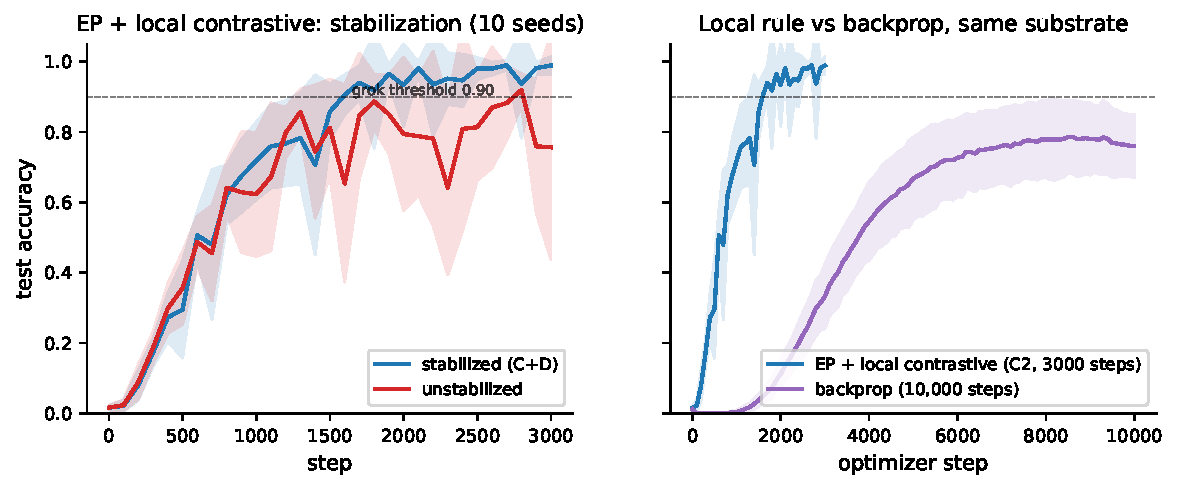
\includegraphics[width=0.62\textwidth]{figures/F1_grokking_curves.pdf}
\caption{Grokking curves (test accuracy vs.\ step, mean $\pm$ std). Left: the stabilized (C2) and unstabilized (C3) multiplication arms, 10 seeds each --- stabilized reaches and holds $\geq 0.90$ (10/10 final, 9/10 by window); unstabilized peaks then collapses (grok-then-forget). Right: the same EP arm (C2, 3000 steps) against the backprop reference arm at extended budget (10{,}000 steps, 10 seeds, same substrate and basis) --- EP groks where backprop has not begun (backprop window mean $0.763 \pm 0.089$, 0/10 persistent grok; \S\ref{sec:limitations}). Sources: \texttt{outputs/basis\_swap\_v13\_mult-stab\_frac80\_L6\_N1536\_T10.json}, \texttt{basis\_swap\_v13\_mult-nostab\_frac80\_L6\_N1536\_T10.json}, and \texttt{outputs/bp\_control\_arm1\_mult\_main\_L6\_N1536\_T10\_S10000\_n10.json} (history fields). The horizontal axis counts optimizer updates; EP updates each incur $T$ settling steps, so this is not forward-compute-matched.}
\label{figslot:f1}
\end{figure}

\begin{figure}[htbp]
\centering
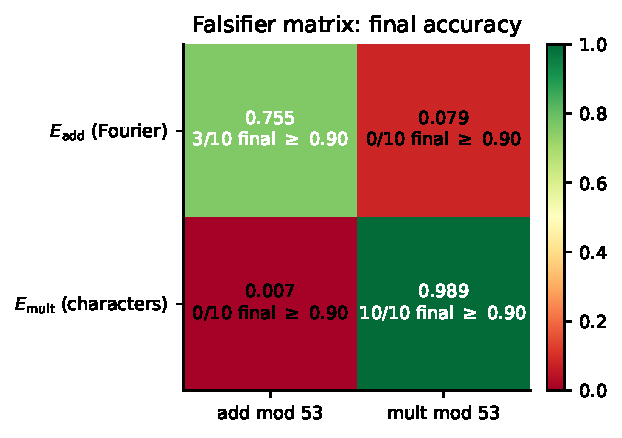
\includegraphics[width=0.5\textwidth]{figures/F2_falsifier_matrix.pdf}
\caption{The $2\times2$ falsifier matrix (final accuracy): $(E_{\mathrm{add}}, \mathrm{add})$ best 9/10, final 3/10; $(E_{\mathrm{add}}, \mathrm{mult})$ 0/10; $(E_{\mathrm{mult}}, \mathrm{mult})$ 10/10; $(E_{\mathrm{mult}}, \mathrm{add})$ 0/10 (all chance, finals 0.002--0.011) --- each basis linearizes exactly one operation. Sources: \texttt{outputs/matched\_add\_L6\_N1536\_T10.json}, \texttt{outputs/matched\_mult\_L6\_N1536\_T10.json}, \texttt{outputs/basis\_swap\_v13\_mult-stab\_frac80\_L6\_N1536\_T10.json}, \texttt{outputs/f2\_emult\_add\_L6\_N1536\_T10.json}.}
\label{figslot:f2}
\end{figure}

\begin{figure}[htbp]
\centering
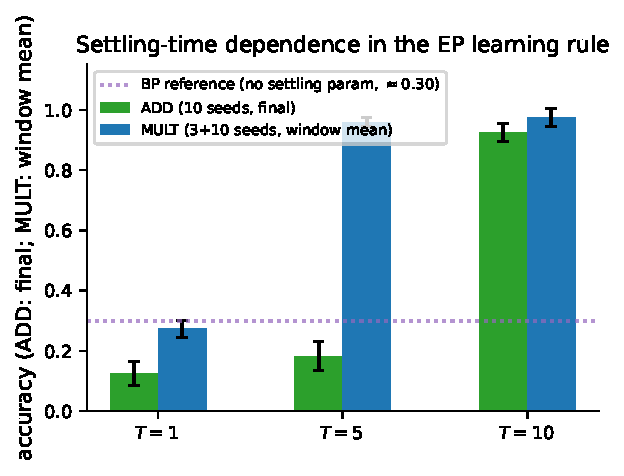
\includegraphics[width=0.6\textwidth]{figures/F3_Tcliff.pdf}
\caption{T-cliff: accuracy vs.\ $T \in \{1,5,10\}$. ADD: 0.125/0.182/0.924 (10 seeds, final). MULT: 0.273/0.959/0.975 window (0.989 final, C2, 10 seeds) --- the cliff occurs at lower $T$ and is complete (0/3$\rightarrow$3/3). BP: 0.300 at all three $T$ (T-inert, 3 seeds --- an existence proof, reported at lower confidence than the $n{=}10$ arms). The gradient quality is highly $T$-sensitive --- a characteristic consequence of the EP settling procedure (backpropagation has no settling-time axis; the contrast is structural; the backprop reference arm, \S\ref{sec:limitations}, does not grok mult within budget on this substrate). Sources: \texttt{outputs/l6eqcap\_T1\_10seeds.json}, \texttt{l6eqcap\_T5\_10seeds.json}, \texttt{l6eqcap\_T10\_10seeds.json} (add, 5ea8114); \texttt{outputs/ep\_mult\_tcliff\_banking\_L6\_N1536.json} (mult, 8cad9ef); \texttt{outputs/bp\_control\_arm1\_mult\_tcliff\_L6\_N1536.json} (BP null, 9c8d686).}
\label{figslot:f3}
\end{figure}

\begin{figure}[htbp]
\centering
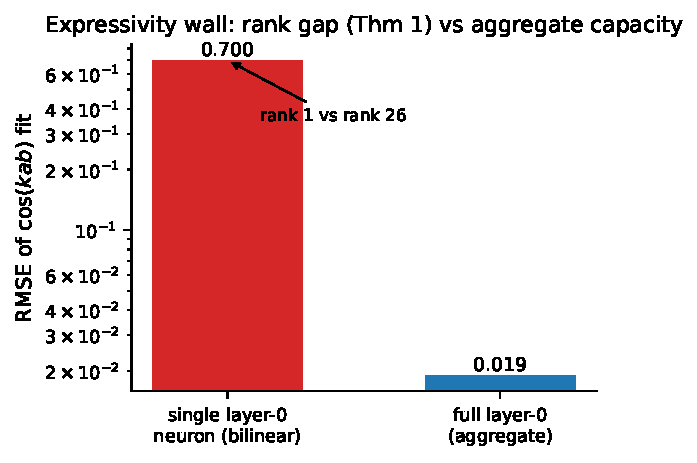
\includegraphics[width=0.55\textwidth]{figures/F4_expressivity.pdf}
\caption{Expressivity: RMSE of the $\cos(kab)$ fit. Best rank-1 separable approximation $\approx 0.69$ ($R^2 < 0.05$); full layer-0 0.019 ($R^2 = 0.999$). Theorem~\ref{thm:rankgap} gives rank $((p+1)/2=27)$ for the full field $\mathbb{F}_p$; the experimentally used nonzero-residue kernel (discrete log undefined at zero) has rank $((p-1)/2=26)$. The two sides of the wall: the neuron's rank gap and the layer's aggregate capacity --- capacity without learnability under the local rule, which still fails to grok in this basis (0/10; \S\ref{sec:falsified}). The single-neuron value is reproduced from the kernel in \texttt{outputs/f4\_expressivity\_audit.json} (RMSE 0.7004, $R^2$ 0.036); the layer-0 empirical fit is documented with provenance in the same file.}
\label{figslot:f4}
\end{figure}

\begin{figure}[htbp]
\centering
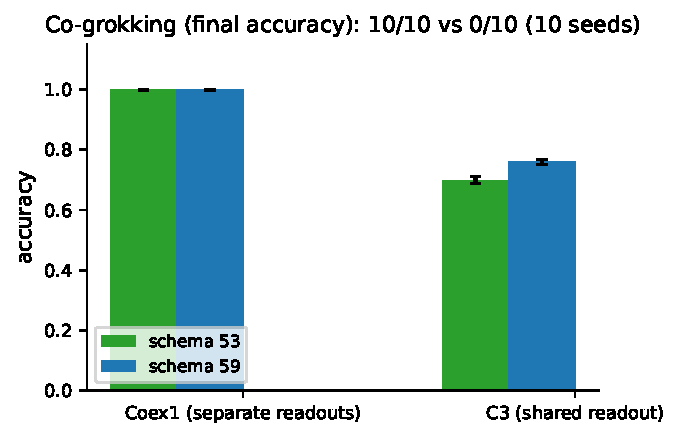
\includegraphics[width=0.6\textwidth]{figures/F5_coexistence.pdf}
\caption{Co-grokking: per-schema accuracy for add mod 53 + add mod 59 (C8, label accuracy-only) and the shared-readout lesion (C9). C8 co-groks 10/10 on accuracy; C9 fails 0/10, localizing separation pressure to the readout. Sources: \texttt{outputs/coex/coex\_Coex1\_10seeds.json} and \texttt{coex/coex\_C3\_10seeds.json}.}
\label{figslot:f5}
\end{figure}

\begin{figure}[htbp]
\centering
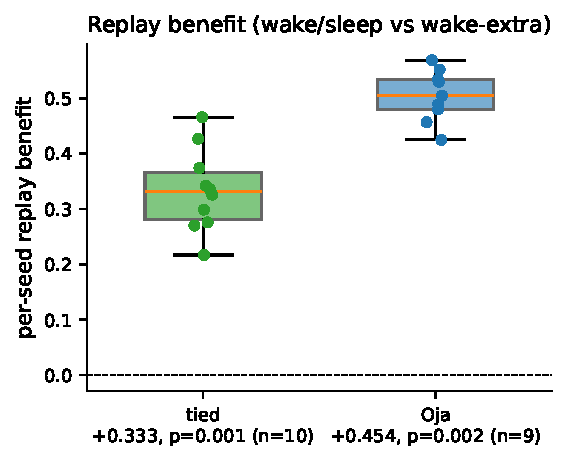
\includegraphics[width=0.55\textwidth]{figures/F6_replay.pdf}
\caption{Replay benefit (C10, corrected): Oja +0.454 (one-sided Wilcoxon $p = 0.002$); tied +0.333 (one-sided $p = 0.001$). Data-quality caveat: oja seed 1's wake arms absent from the source log, $n{=}9$ for the Oja comparison. Source: \texttt{outputs/mvp0\_replay\_10seeds.json} (converted from \texttt{outputs/results\_10seed.txt}, 3745dbf).}
\label{figslot:f6}
\end{figure}

\paragraph{Code availability}
The engine, experiment runner, and all result artifacts needed to reproduce the headline result are available in the public repository accompanying this paper (\url{https://github.com/xmucane-ai/ep-oja-grokking-mult}). The repository contains the engine and run scripts (cleaned, without full history), the 10-seed result JSONs for every claim in Appendix~\ref{app:claims}, and a README with the exact reproduce commands. Repository code is MIT-licensed (paper text \copyright{} the author; third-party PDFs \copyright{} their respective authors, included for review convenience only).

\paragraph{Use of AI tools}
The author used AI assistants throughout the research and writing process: for experiment execution and debugging, for mathematical verification, for literature search, and for drafting and editing prose. AI-based review agents were additionally used to stress-test the paper; their findings were treated as advisory and checked by the author against the committed artifacts, and the paper's central proof was re-derived by hand. All experiments were run by the author's own code, and every claim in this paper was checked by the author against the committed artifacts --- including several corrections made during review (e.g., the $p{=}97$ chance-baseline label, the C11 whitening-gap status, and the $R_{\mathrm{cap}}$ capacity classification at $N{=}512$). The author takes full responsibility for the content of this paper.

\bibliographystyle{plain}
\begin{thebibliography}{18}

\bibitem{power2022}
A.~Power, Y.~Burda, H.~Edwards, I.~Babuschkin, and V.~Misra.
\newblock Grokking: Generalization beyond overfitting on small algorithmic datasets.
\newblock \emph{arXiv:2201.02177}, 2022.

\bibitem{nanda2023}
N.~Nanda, L.~Chan, T.~Lieberum, J.~Smith, and J.~Steinhardt.
\newblock Progress measures for grokking via mechanistic interpretability.
\newblock \emph{arXiv:2301.05217}, 2023.

\bibitem{nguyen2026}
H.~D. Nguyen.
\newblock The discrete-log clock: How a transformer learns modular multiplication.
\newblock \emph{arXiv:2606.17399}, 2026 (ICML).

\bibitem{gromov2023}
A.~Gromov.
\newblock Grokking modular arithmetic.
\newblock \emph{arXiv:2301.02679}, 2023.

\bibitem{doshi2024}
S.~Doshi, D.~He, A.~Das, and A.~Gromov.
\newblock Grokking modular polynomials.
\newblock \emph{arXiv:2406.03495}, 2024.

\bibitem{scellier2017}
B.~Scellier and Y.~Bengio.
\newblock Equilibrium propagation: Bridging the gap between energy-based models and backpropagation.
\newblock \emph{Frontiers in Computational Neuroscience}, 11:24, 2017.

\bibitem{hoier2023}
R.~H{\o}ier, C.~Staudt, and C.~Zach.
\newblock Dual propagation: Accelerating contrastive Hebbian learning with dyadic neurons.
\newblock \emph{ICML 2023}, PMLR 202:13141--13156; \emph{arXiv:2302.01228}.

\bibitem{hoier2024}
R.~H{\o}ier and C.~Zach.
\newblock Two tales of single-phase contrastive Hebbian learning.
\newblock \emph{ICML 2024}, PMLR 235:18470--18488; \emph{arXiv:2402.08573}.

\bibitem{sacramento2018}
J.~Sacramento, R.~P.~Costa, Y.~Bengio, and W.~Senn.
\newblock Dendritic cortical microcircuits approximate the backpropagation algorithm.
\newblock \emph{NeurIPS 2018}.

\bibitem{raoballard1999}
R.~P.~N. Rao and D.~H. Ballard.
\newblock Predictive coding in the visual cortex: A functional interpretation of some extra-classical receptive-field effects.
\newblock \emph{Nature Neuroscience}, 2:79--87, 1999.

\bibitem{olshausen1996}
B.~A. Olshausen and D.~J. Field.
\newblock Emergence of simple-cell receptive field properties by learning a sparse code for natural images.
\newblock \emph{Nature}, 381:607--609, 1996.

\bibitem{urbanczik2014}
R.~Urbanczik and W.~Senn.
\newblock Learning by the dendritic prediction of somatic spiking.
\newblock \emph{Neuron}, 81:521--528, 2014.

\bibitem{guerguiev2017}
J.~Guerguiev, T.~P. Lillicrap, and B.~A. Richards.
\newblock Towards deep learning with segregated dendrites.
\newblock \emph{eLife}, 6:e22901, 2017.

\bibitem{oja1982}
E.~Oja.
\newblock Simplified neuron model as a principal component analyzer.
\newblock \emph{Journal of Mathematical Biology}, 15:267--273, 1982.

\bibitem{innocenti2025}
M.~Innocenti, E.~Achour, and C.~L. Buckley.
\newblock $\mu$PC: Parameterization matters for predictive coding.
\newblock \emph{NeurIPS 2025}; \emph{arXiv:2505.13124}.

\bibitem{seely2026}
N.~Seely and N.~Gould.
\newblock Predictive coding at any depth (PC-ALM).
\newblock \emph{arXiv:2605.31022}, 2026.

\bibitem{lv2025}
L.~Lv et al.
\newblock Dendritic localized learning.
\newblock \emph{PMLR v267/lv25c}, 2025; \emph{arXiv:2501.09976}.

\bibitem{zunkovic2024}
B.~Zunkovi{\'c} and E.~Ilievski.
\newblock Grokking phase transitions in learning local rules.
\newblock \emph{JMLR 22-1228}, 2024; \emph{arXiv:2210.15435}.
\newblock (``local'' here means data-local rule learning; cited only to disambiguate from biologically-plausible local learning.)

\end{thebibliography}

\end{document}
